\section{Fiber RX}

The fiber receive interface (figure \ref{fiberrx} ) is in some ways
simpler than the transmit interface. The interface's state machine
(Figure \ref{}) waits until we receive a new packet with no errors and
the appropriate K-character, and then sets about latching the relevant
input words.

\begin{figure}[h!]
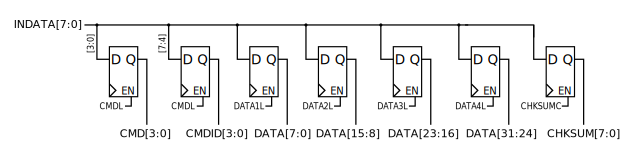
\includegraphics[scale=1.0]{fiberRX.svg}
\label{fiberrx}
\caption{The Fiber Reception interface}. 
\end{figure}


Any error in 8b/10b decoding or spurious (out-of-sequence) comma
character causes a transition back to \state{NONE}, preventing the
reception of an invalid data frame.


\subsection{Decoder}

The deserialization step is somewhat more difficult; as the core is
running at 72 MHz, we can oversample the input bitstream by a factor
of 9. The 8b/10b encoding guarantees a maximum run of five, so we
simply need to maintain a lock for at most five input-bit-cycles.

\begin{figure}[h!]
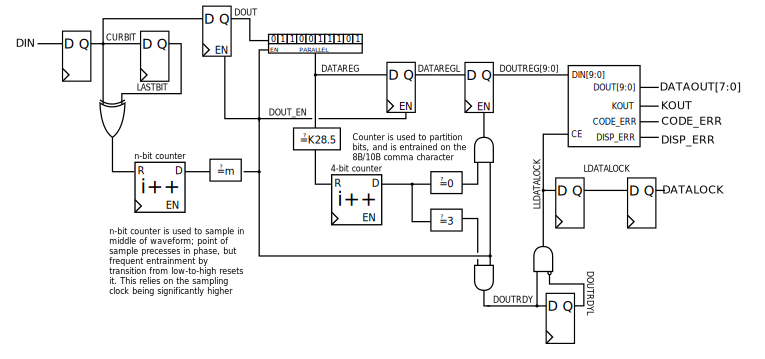
\includegraphics[scale=1.0]{decoder.svg}
\label{decoder}
\caption{The oversampling fiber decoder}
\end{figure}

The decoder used here (figure \ref{decoder}) is generalized to work
for different oversampling rates, as it was not known in the early
stage of development what the final oversampling rate would be. We use
a counter which is reset on each bit transition, and shift in the
relevant bits; in the absence of transitions the counter loops and
appropriately samples.

The detection of the unique K28.5 comma character is used to partition
the bits into words via the serial-to-paralllel shift register
\signal{DATAREG}. From that point on we simply count in multiples of
10 bits in gating the output into the 8b/10b decoder.



